\documentclass[twoside,10pt]{report}
\usepackage{/Users/bradenhoagland/latex/styles/toggles}
%\toggletrue{sectionbreaks}
\newcommand{\docTitle}{Stochastic Calculus}
\usepackage{/Users/bradenhoagland/latex/styles/common}
\importStyles{formal}{rainbow}{boxy}

%\renewcommand{\theenumi}{\alph{enumi}}

\begin{document}
%\tableofcontents

%+-------------------+
%| +---------------+ |
%| |    Chapter    | |
%| +---------------+ |
%+-------------------+
% Basics

\chapter{Basics}

\warn{variation, quadratic variation}

\warn{filtration}

%+-------------------+
%| +---------------+ |
%| |    Chapter    | |
%| +---------------+ |
%+-------------------+
% Brownian Motion

\chapter{Brownian Motion}

\begin{defn}[]
A standard \textbf{Brownian motion} $B(t,\omega)$ is a continuous time $\R$-valued stochastic process over some $(\Omega,\mathcal{F},\mathbb{P})$ such that
\begin{enumerate}
	\item $B_{t}-B_{s}\sim \mathcal{N}(0, t-s)$;
	\item Disjoint increments are independent;
	\item The sample path $t \mapsto B_{t}(\omega)$ is continuous with probability 1.
\end{enumerate}
\end{defn}

At all times, a Brownian motion receives an infinitesimal Gaussian kick. The intuition here is that ``$dB$" is then a Gaussian random variable. Of course, $dB$ is meaningless right now since $B$ is nowhere differentiable with probability 1, but we will give it meaning later in terms of It\^o integrals, and the interpretation will be the same.

\begin{figure}[H]
	\centering
	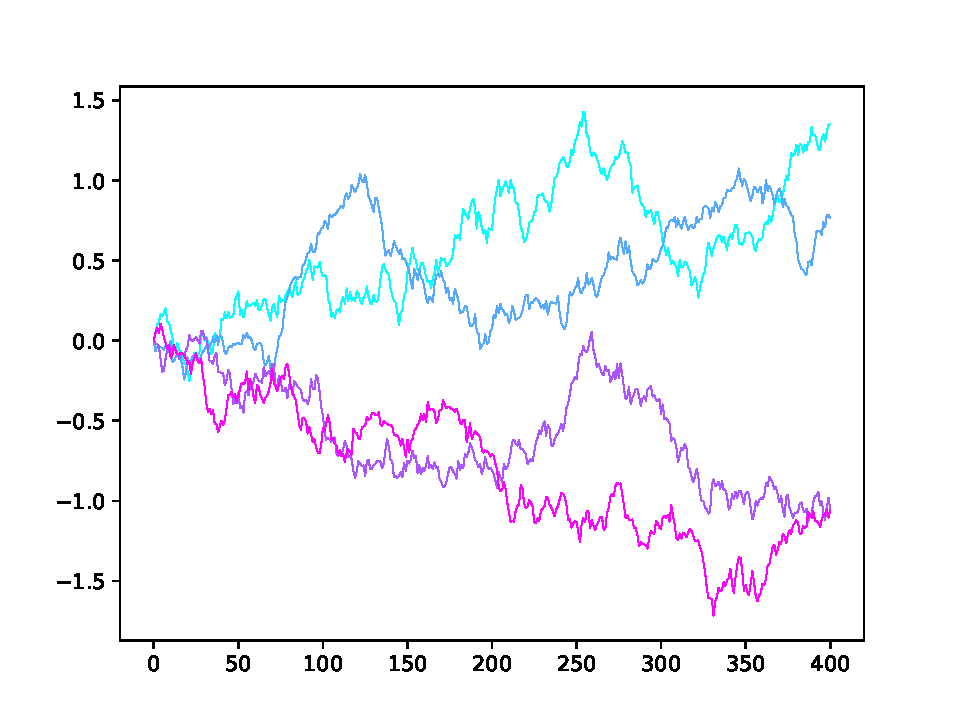
\includegraphics[scale=0.7]{fig/brownian.pdf}
	%\caption{}
\end{figure}

\begin{prop}
	If $B_{t}$ is a Brownian motion, then so are the following two processes:
	\begin{itemize}
		\item $X_{t} := \frac{1}{\sqrt{\alpha} } B_{\alpha t}$ for fixed $\alpha > 0$;
		\item $Y_{t} := B_{s+t} - B_{s}$ for fixed $s>0$;
		\item $Z_{t} := t B_{1/t}$.
	\end{itemize}
\end{prop}

A useful fact for proving that disjoint intervals are independent: two Gaussians are independent $\iff$ they have 0 covariance.

\begin{prop}
If $B_{t}$ is a Brownian motion, then $\cov(B_{t},B_{s}) = \min(t,s)$.
\end{prop}

\warn{Construct a BM using Wiener measure and $B_{t}(\omega) = \omega_{t}$.}

Let $ A := \left\{ \omega \;|\; B_{t_k}(\omega) \in (a_{k},b_{k}) \text{ for } k=1,\dots,N \right\}$. If
\[
\phi(s,y) := \frac{\exp\left( -y^2/(2s) \right)}{\sqrt{2 \pi s^2} } ,
\] then the probability of $A$ is
\[
\P{ A } = \int_{a_1}^{b_1} \cdots \int_{a_n}^{b_n} \phi(t_1, x_1) \prod_{i=2}^{N} \phi(t_{i}-t_{i-1},x_{i}-x_{i-1}) \; dx_1\;\cdots\; dx_{n}.
\] The idea here is that $\phi(t_{i}-t_{i-1},x_{i}-x_{i-1})$ is the conditional density for $B_{t_k}$ given $B_{t_{k-1}}=x_{k-1}$.

\begin{defn}[]
A function $f:I\to \R$ is $\gamma$-\textbf{H\"older continuous} if there is a $C < \infty$ such that
\[
|f(t) - f(s)| \leq C \; |t-s|^{\gamma}
\] for all $s,t \in I$. Functions with $\gamma=1$ are \textbf{Lipschitz continuous}.
\end{defn}

\begin{thrm}[Kolmogorov Continuity Theorem]
	Let $\left\{ X_{t} \right\}$ be a stochastic process on $[0,1]$. If there are $\alpha,\beta,C>0$ such that
	\[
	\E{ |X_{t}-X_{s}|^{\alpha} } \leq C |t-s|^{1+\beta},
	\] then there is a version $\tilde{X}_{t}$ of $X_{t}$ with sample paths that are almost surely $\gamma$-H\"older continuous for $\gamma \in (0, \beta/\alpha)$.
\end{thrm}

\warn{version means $\P{ \tilde{X}_{t}=X_{t} }=1$ for all $t$.}

This implies that the sample paths of Brownian motion are almost surely H\"older continuous for $\gamma \in (0,1/2)$.

\begin{prop}
If $B$ is a Brownian motion on $[0,T]$, then with probability 1,
\begin{itemize}
	\item $V^{p}(B,[0,T]) < \infty$ for $p>2$;
	\item $V^{p}(B,[0,T]) = \infty$ for $p<2$.
\end{itemize}
The quadratic variation of $B$ is $[B,B](t) = t$.
\end{prop}


\end{document}
